\section{Graphene, nanotubes and quantum dots}\label{sec:16.3}

An electron of a graphene sheet that receives more than the work function, about \SI{4.3}{eV}, can leave the sheet without meeting another atom. It then carries into the vacuum the direction and the energy the dark matter gave it, and both can be measured. A bulk crystal turns the same deposit into a cascade of secondary pairs and phonons, and the direction is lost. Carbon nanotubes keep the one-atom thickness and roll the sheet into a cylinder of radius $r_{\mathrm{t}}$. Rolling the sheet quantizes the momentum around the tube and opens a gap in most nanotubes. Quantum dots, nanocrystals a few nanometers across, push confinement to all three directions: a lead sulfide dot \SI{3.3}{nm} across has an optical gap of \SI{1.2}{eV}, against \SI{0.41}{eV} for the bulk crystal, and it re-emits the energy of a pair as a photon~\cite{blanco2023dark}.

\subsection{Electron ejection into vacuum}\label{sec:16.3-ejection}

Take an electron in band $i$ with in-plane crystal momentum $\vect{k}_\parallel$, bound by $E_B(i,\vect{k}_\parallel) \ge 0$ below the Fermi level. It leaves with kinetic energy $E_{\mathrm{ej}} = p_{\mathrm{ej}}^2/2m_e$ when the dark matter deposits
\begin{equation}
  \omega = E_{\mathrm{ej}} + \Phi_{\mathrm{wf}} + E_B(i,\vect{k}_\parallel) ,
  \label{eq:16.3-omega}
\end{equation}
with $\Phi_{\mathrm{wf}}$ the work function, the energy from the Fermi level to the vacuum. For graphene $\Phi_{\mathrm{wf}} \simeq \SI{4.3}{eV}$, and it can be moved by the choice of substrate~\cite[text after Eq.~(5) and footnote~2]{hochberg2017directional}. The largest energy a particle can deposit is its kinetic energy, $\mchi v_{\mathrm{max}}^2/2$, so ejection starts at $\mchi = 2\Phi_{\mathrm{wf}}/v_{\mathrm{max}}^2 = \SI{1.22}{MeV}$, at a momentum transfer of at least $\Phi_{\mathrm{wf}}/v_{\mathrm{max}} = \SI{1.62}{keV}$. This minimum momentum transfer is already a fifth of the momentum scale of a carbon $2p$ orbital, $\beta = Z_{\mathrm{eff}}/2a_0 = \SI{7.51}{keV}$ for the hydrogenic orbital with $Z_{\mathrm{eff}} = 4.03$ that Hochberg et al.\ fit to the overlap of neighboring orbitals~\cite[Eq.~(2)]{hochberg2017directional}. Ejection probes the short-distance structure of the orbitals, as atomic ionization does (\cref{sec:2.2}), and not their tails.

In the independent-particle picture the initial states are the occupied Bloch states $\psi_{i\vect{k}_\parallel}$ of the $\pi$ band and the three $\sigma$ bands, normalized over the sample, and each final state is a hole in the sheet with a free electron. We take the free electron as a plane wave $\ee^{\ii\vect{p}\cdot\vect{r}}/\Vol^{1/2}$ of momentum $\vect{p}$, $|\vect{p}| = p_{\mathrm{ej}}$. Its transition form factor \cref{eq:2.2-ff} is the momentum-space wavefunction of the initial state, $M_{\mathrm{PW}}(\vect{p},\vect{q}) = \tilde\psi_{i\vect{k}_\parallel}(\vect{p} - \vect{q})$, and the structure factor of \cref{eq:4.2-Sab} becomes
\begin{equation}
  S_{\mathrm{ej}}(\vect{q},\omega) = \frac{2\pi}{\Vol}\sum_{i,\vect{k}_\parallel,\sigma}\int\frac{\dd^3p}{(2\pi)^3}\,|M(\vect{p},\vect{q})|^2\,\delta\bigl(\omega - E_{\mathrm{ej}} - \Phi_{\mathrm{wf}} - E_B(i,\vect{k}_\parallel)\bigr) ,
  \label{eq:16.3-Sej}
\end{equation}
with $M = M_{\mathrm{PW}}$ for plane waves and $\sigma$ the spin. Only energy is conserved. Since the bound state is not a momentum eigenstate, it supplies whatever part of $\vect{q}$ the electron does not leave with, and $\vect{p}$ and $\vect{q}$ are independent variables. Inserting \cref{eq:16.3-Sej} and $|\tilde V|^2 = \pi\sigmae\FDM^2/\mu_{\chi e}^2$ (\cref{eq:1.4-Vsq}) into \cref{eq:8.2-spectrum}, with $\rho_T\Vol = N_{\mathrm{cell}}M_{\mathrm{cell}}$, the factors $2\pi\cdot\pi/(2\pi)^3$ combine into $1/4\pi$, and the rate per unit mass is a sum of cross-sections, one for each occupied state:
\begin{equation}
  \begin{gathered}
  \mathcal{R} = \frac{\rho_\chi}{\mchi\,N_{\mathrm{cell}}M_{\mathrm{cell}}}\sum_{i,\vect{k}_\parallel,\sigma}\int\dd^3v\,f_\chi(\vect{v})\,\langle\sigma v\rangle_{i\vect{k}_\parallel}(\vect{v}) ,\\
  \langle\sigma v\rangle_{i\vect{k}_\parallel} = \frac{\sigmae}{\mu_{\chi e}^2}\int\frac{\dd^3p}{(2\pi)^3}\int\frac{\dd^3q}{4\pi}\,\FDM(q)^2\,|M(\vect{p},\vect{q})|^2\,\delta\Bigl(E_{\mathrm{ej}} + \Phi_{\mathrm{wf}} + E_B + \frac{q^2}{2\mchi} - \vect{q}\cdot\vect{v}\Bigr) .
  \end{gathered}
  \label{eq:16.3-rate}
\end{equation}
For plane waves the cross-section is that of Hochberg et al.~\cite[Eq.~(5)]{hochberg2017directional}. They write the sum over states as $2N_{\mathrm{C}}A_{\mathrm{cell}}\int\dd^2k_\parallel/(2\pi)^2$ per band, with $N_{\mathrm{C}}$ the number of carbon atoms per unit mass and $A_{\mathrm{cell}}$ the area of the unit cell. They take for $\tilde\psi$ the tight-binding function of one atom and its three nearest neighbors~\cite[Eqs.~(1), (3), (7)]{hochberg2017directional}. A nanotube changes only the sum over states. Going once around the tube must return the Bloch phase, so the momentum around the circumference takes the values $n/r_{\mathrm{t}}$. Then $A_{\mathrm{cell}}\int\dd^2k_\parallel/(2\pi)^2$ becomes $(A_{\mathrm{cell}}/2\pi r_{\mathrm{t}})\sum_n\int\dd k_z/2\pi$, with $k_z$ along the axis; with this sum over states, \cref{eq:16.3-rate} is the rate of Cavoto et al.~\cite[Eqs.~(16)--(18), (23)]{cavoto2018sub}.

With Bloch states, the in-plane part of $\vect{p} - \vect{q}$ is fixed up to a reciprocal-lattice vector by the crystal momentum of the hole. A Bloch state normalized over $N_{\mathrm{cell}}$ cells has $|\tilde\psi_{i\vect{k}_\parallel}(\vect{k})|^2 \propto \sum_{\vect{G}}\delta^2(\vect{k}_\parallel' - \vect{k}_\parallel - \vect{G})$, with $\vect{k}_\parallel'$ the in-plane part of $\vect{k}$. As a result, each direction of the ejected electron selects one state of each band, with its own binding energy. The selection of one state per band is the origin of the diffraction pattern that Hochberg et al.\ find in the angular distribution of electrons ejected by a cold stream~\cite[Sect.~III]{hochberg2017directional}. The halo washes the pattern out but keeps the forward peak: the momentum-space orbital is largest when $\vect{p} - \vect{q}$ is small, and the electron leaves close to the direction of $\vect{q}$, which follows the dark-matter velocity. For the standard halo they find the forward rate about twice the backward rate between \SI{10}{MeV} and \SI{10}{GeV}~\cite[Sect.~III]{hochberg2017directional}, and the daily rotation of a fixed sheet modulates both rates.

The orbitals and the binding energies are the material input. They come from a density-functional ground state, with maximally localized Wannier functions for the occupied bands and an all-electron orbital for the carbon 1s shell, which a pseudopotential lacks (\cref{app:E.21}).

\paragraph{Orthogonality of the final state.} A plane wave is not an eigenstate of the sheet, and it is not orthogonal to the state the electron leaves. As $q \to 0$, $M_{\mathrm{PW}}$ tends to $\tilde\psi_{i\vect{k}_\parallel}(\vect{p})$, which is not zero, so plane waves predict ejection with no momentum transfer, although $\ee^{\ii\vect{q}\cdot\vect{r}} \to 1$ cannot connect two orthogonal eigenstates. The cure is to orthogonalize the final state to the occupied states, $|\chi_{\vect{p}}\rangle = |\vect{p}\rangle - \sum_n|\psi_n\rangle\langle\psi_n|\vect{p}\rangle$, the orthogonalized plane wave (OPW). Its transition form factor is
\begin{equation}
  M_{\mathrm{OPW}}(\vect{p},\vect{q}) = \tilde\psi_i(\vect{p} - \vect{q}) - \sum_{n\in\mathrm{occ}}\tilde\psi_n(\vect{p})\,f_{i\to n}(\vect{q}) ,
  \label{eq:16.3-opw}
\end{equation}
with $f_{i\to n}$ the form factor \cref{eq:2.2-ff} between occupied states, here written with a single index for $(i,\vect{k}_\parallel)$. Since $f_{i\to n}(\vect{q}) = \delta_{in} + O(q)$, the term without momentum transfer cancels and $M_{\mathrm{OPW}} = O(q)$. To size the orthogonalization correction we take the hydrogenic $2p_z$ orbital above, $\psi \propto r\ee^{-\beta r}\cos\theta$ with $\tilde\psi(\vect{k}) \propto \beta k_z/(\beta^2 + k^2)^3$~\cite[Eq.~(4)]{hochberg2017directional}, orthogonalize the plane wave to it alone, and average over the orientation of the sheet. Integrated over the directions of the ejected electron, $|M_{\mathrm{OPW}}|^2/|M_{\mathrm{PW}}|^2$ runs from 0.46 to 25 at $E_{\mathrm{ej}} = 50$ to \SI{100}{eV} and $q = 5$ to \SI{40}{keV}. The ratio depends on $q$ and on the angle between $\vect{q}$ and the orbital axis, and an orbital of the same form with the more diffuse exponent $1.568/a_0$ of Clementi and Raimondi gives 0.4 to 4.3. At \SI{10}{eV} it reaches 740, but only at $q \gg p_{\mathrm{ej}}$, where the plane-wave amplitude has already fallen as $|\vect{p} - \vect{q}|^{-5}$ and contributes little. The rate weights each $(\vect{p},\vect{q})$ by the halo, so these ratios bound the correction without giving it.

For an orbital averaged over orientations, $|M|^2$ integrated over the directions of $\vect{p}$ depends only on $p_{\mathrm{ej}}$ and $q$. Call this integral $K(p_{\mathrm{ej}},q)$. The velocity integral of \cref{eq:16.3-rate} then reduces with \cref{eq:A.8-eta}, $\int\dd^3q\,g(q)\int\dd^3v\,f_\chi\,\delta(\cdots) = 2\pi\int q\,\dd q\,\eta(\vmin)\,g(q)$, and $p^2\dd p = m_ep_{\mathrm{ej}}\,\dd E_{\mathrm{ej}}$ gives the spectrum per electron
\begin{equation}
  \frac{\dd\langle\sigma v\rangle}{\dd E_{\mathrm{ej}}} = \frac{\sigmae\,m_e\,p_{\mathrm{ej}}}{16\pi^3\mu_{\chi e}^2}\int q\,\dd q\,\eta\bigl(\vmin(q,\omega)\bigr)\,\FDM(q)^2\,K(p_{\mathrm{ej}},q) ,
  \label{eq:16.3-iso}
\end{equation}
with $\vmin = \omega/q + q/2\mchi$ and $\omega$ from \cref{eq:16.3-omega}. Summed over the electrons of a full atomic shell with plane waves, \cref{eq:16.3-iso} times $E_{\mathrm{ej}}$ is \cref{eq:2.2-ion} with \cref{eq:2.2-fion-pw}. \Cref{fig:16-ejection} applies it to the $\pi$ electrons of graphene, one per atom, with the momentum density of the isolated orbital. Their binding energies are those of the nearest-neighbor band, $E_B = t|1 + \ee^{\ii\vect{k}\cdot\vect{a}_1} + \ee^{\ii\vect{k}\cdot\vect{a}_2}|$ with $\vect{a}_{1,2}$ the primitive vectors and hopping $t = \SI{2.8}{eV}$~\cite[text after Eq.~(5)]{castroneto2009electronic}, spread from 0 to \SI{8.4}{eV} with a mean of \SI{4.41}{eV}. At $\sigmae = \SI{e-37}{cm^2}$ and a heavy mediator the $\pi$ electrons alone give \num{6.9e3} events per kg-year at \SI{10}{MeV} with plane waves and \num{1.0e4} with orthogonalized ones; at \SI{100}{MeV}, \num{2.8e3} and \num{5.2e3}. The orthogonalization raises the rate, by factors of 1.44 and 1.84, and moves the peak of the spectrum up in energy. For a light mediator the factors are only 1.14 and 1.19. The light mediator weights the smallest momentum transfers, a few keV, where the orthogonality term lowers the squared amplitude (to 0.46--0.74 of the plane-wave value at $q = \SI{5}{keV}$ for $E_{\mathrm{ej}} = \SI{50}{eV}$) and so partly cancels the gain at larger $q$.

\begin{figure}[tbp]
  \centering
  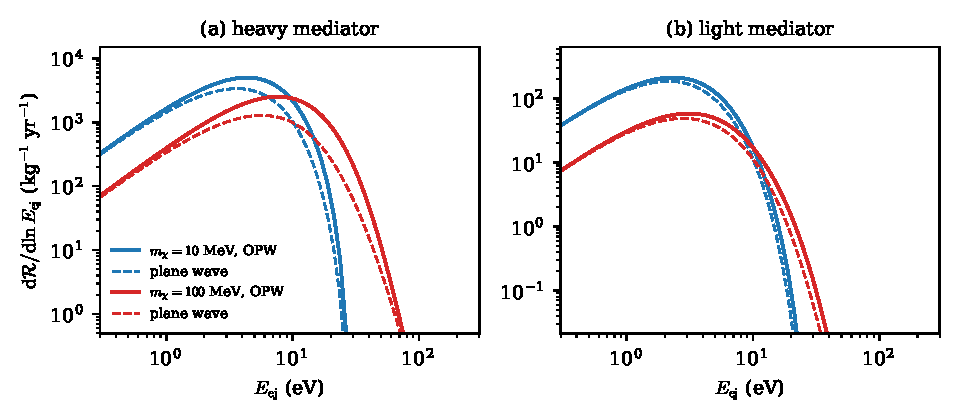
\includegraphics[width=\linewidth]{figures/ch16/fig16_3.pdf}
  \caption{Ejection spectra of the $\pi$ electrons of graphene, $\dd\mathcal{R}/\dd\ln E_{\mathrm{ej}}$ per kg-year at $\sigmae = \SI{e-37}{cm^2}$, against the kinetic energy $E_{\mathrm{ej}}$ of the ejected electron, for $\mchi = \SI{10}{MeV}$ (blue) and \SI{100}{MeV} (red): (a) heavy mediator, $\FDM = 1$; (b) light mediator, $\FDM = (\alpha m_e/q)^2$. Dashed: plane-wave final states; solid: final plane wave orthogonalized to the initial orbital, \cref{eq:16.3-opw}. Model: one hydrogenic $2p_z$ orbital per atom with $Z_{\mathrm{eff}} = 4.03$, Bloch interference between neighbors dropped, binding energies of the nearest-neighbor $\pi$ band ($t = \SI{2.8}{eV}$, 0 to \SI{8.4}{eV}), work function \SI{4.3}{eV}, sheet orientation averaged, standard halo of \cref{tab:1-shm}. The $\sigma$ electrons are not included.}
  \label{fig:16-ejection}
\end{figure}

\begin{limitbox}[Vacuum ejection with plane-wave final states][lim:16.3a]
The ejection rate of a sheet or a tube with plane-wave final states, $M = \tilde\psi_{i\vect{k}_\parallel}(\vect{p} - \vect{q})$ in \cref{eq:16.3-rate}, is the published form~\cites[Eqs.~(5), (7)]{hochberg2017directional}[Eq.~(23)]{cavoto2018sub}.
\par\smallskip
{\centering
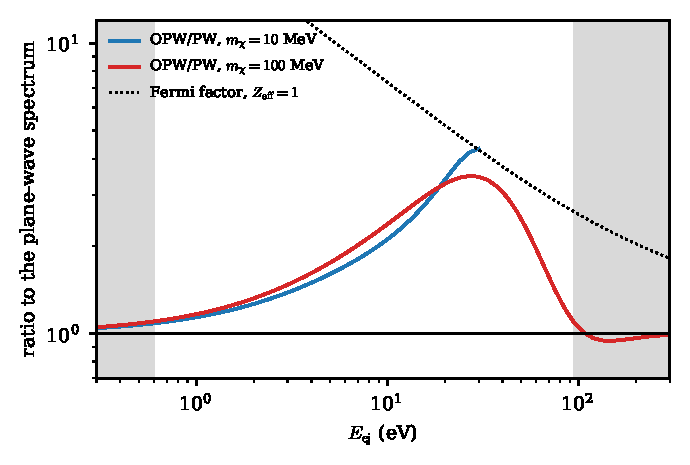
\includegraphics[width=0.85\linewidth]{figures/ch16/limit16_3a.pdf}
\captionof{figure}{Ejection spectrum of graphene $\pi$ electrons with orthogonalized final states, \cref{eq:16.3-opw}, divided by the plane-wave spectrum, against the kinetic energy $E_{\mathrm{ej}}$ of the ejected electron, for $\mchi = \SI{10}{MeV}$ (blue, which ends at \SI{31}{eV}) and \SI{100}{MeV} (red), heavy mediator, in the model of \cref{fig:16-ejection}. Thin line: the plane-wave form. Dotted: the Fermi factor \cref{eq:2.2-fermi} with $Z_{\mathrm{eff}} = 1$, the largest final-state enhancement an unscreened hole can produce. Gray: the orthogonalized spectrum within \SI{10}{\percent} of the plane-wave one, $E_{\mathrm{ej}} < \SI{0.60}{eV}$ and, for \SI{100}{MeV}, $E_{\mathrm{ej}} > \SI{94}{eV}$.}\label{fig:16-limit-ejection}
\par}
\smallskip
Between these energies, where most of the rate lies, orthogonality raises the spectrum by factors up to 3.5 at \SI{100}{MeV} (2.1 at \SI{10}{eV} and 4.3 at the kinematic end for \SI{10}{MeV}), and the attraction of the hole can add up to the Fermi factor, 7.3 at \SI{10}{eV} and 2.6 at \SI{100}{eV}; neither factor is fixed until all occupied orbitals and true scattering states are used.
\end{limitbox}

The second correction to the plane-wave rate is the final-state interaction. The ejected electron leaves a hole behind, and an unscreened point charge would enhance the slow part of the spectrum by the Fermi factor \cref{eq:2.2-fermi}, 7.3, 3.4 and 2.6 at $E_{\mathrm{ej}} = 10$, 50 and \SI{100}{eV}. Graphene screens the hole with its own electrons, and this screening pushes the factor toward one, and the ejected electron travels only atomic distances near the nuclei before it is in vacuum; for these two reasons Hochberg et al.\ leave the factor out~\cite[text after Eq.~(6)]{hochberg2017directional}. A semiconducting tube screens less. The two corrections cannot simply be multiplied: an orthogonalized plane wave is not a scattering state of the hole, and multiplying it by a Fermi factor counts part of the same distortion twice. The consistent final state is a scattering state of the sheet's own potential plus the screened hole.

\subsection{Semiconducting nanotubes}\label{sec:16.3-tubes}

Below the work function a tube responds through pairs within its own bands. Rolling the sheet quantizes the momentum around the circumference in steps of $1/r_{\mathrm{t}}$, and the Dirac cones of graphene are cut along lines. A tube is metallic when a line passes through a Dirac point; otherwise the nearest line misses it by a third of the spacing, and the subbands, labeled $n$, are massive Dirac bands in one dimension with half-gaps $\Delta_n = nv_{\mathrm{D}}/3r_{\mathrm{t}}$ for $n = 1, 2$. With the velocity $v_{\mathrm{D}} = \num{3.02e-3}$ of \cref{sec:16.2}, or \SI{9.1e5}{m.s^{-1}}, a tube \SI{1}{nm} across has $2\Delta_1 = \SI{0.80}{eV}$. The edge is reached through momentum across the tube, which the structure factor \cref{eq:16.2-embed} does not see except through $|F_\perp|^2 = J_0(q_\perp r_{\mathrm{t}})^2$. At the edge $q_\parallel = 0$ and $\omega = 2\Delta_n$, and since $q \ge \omega/v_{\mathrm{max}}$ the dark matter needs $q_\perp \ge 2\Delta_n/v_{\mathrm{max}}$, that is $q_\perp r_{\mathrm{t}} \ge 2nv_{\mathrm{D}}/3v_{\mathrm{max}}$, independent of the radius: 0.76 for the first subband, where $J_0^2 = 0.74$, and 1.52 for the second, where $J_0^2 = 0.25$. For a \SI{1}{nm} tube the first edge opens at $\mchi = 4\Delta_1/v_{\mathrm{max}}^2 = \SI{226}{keV}$.

Each subband pair is $h = v_{\mathrm{D}}k\sigma_x + \Delta_n\sigma_z$, the one-dimensional form of \cref{eq:7.3-H}, with $k$ along the axis and $g_{\mathrm{deg}} = 4$ for spin and valley. The interband response per unit length follows from two symmetries before any integral is done. The model is invariant under Lorentz boosts with $v_{\mathrm{D}}$ in place of the speed of light, and its density is the time component of a conserved current. The response then has the form $q_\parallel^2\,\mathfrak{p}(s)$, with $s = \omega^2 - v_{\mathrm{D}}^2q_\parallel^2$ the invariant of \cref{sec:7.3} and $\mathfrak{p}$ a function of $s$ alone, and it is enough to compute the response at small $q_\parallel$. There the pair is made at $\pm k$ with $\omega = 2\varepsilon_k$, $\varepsilon_k = (v_{\mathrm{D}}^2k^2 + \Delta_n^2)^{1/2}$. The spinors of the two bands are rotated by the angle $\theta_k$ with $\tan\theta_k = v_{\mathrm{D}}k/\Delta_n$, and the interband overlap is $|\langle +,k + q_\parallel|-,k\rangle|^2 = \tfrac14(\partial_k\theta_k)^2q_\parallel^2 = q_\parallel^2v_{\mathrm{D}}^2\Delta_n^2/4\varepsilon_k^4$. Inserting it in $-\Imag\tilde R = (g_{\mathrm{deg}}/2)\int\dd k\,|\langle +|-\rangle|^2\,\delta(\omega - \varepsilon_k - \varepsilon_{k+q_\parallel})$, summing the two roots and replacing $\omega^2$ by $s$,
\begin{equation}
  -\Imag\tilde R^{\mathrm{1D}}_n(q_\parallel,\omega) = \frac{2g_{\mathrm{deg}}v_{\mathrm{D}}q_\parallel^2\Delta_n^2}{s^{3/2}\,(s - 4\Delta_n^2)^{1/2}}\,\Theta(s - 4\Delta_n^2) .
  \label{eq:16.3-R1D}
\end{equation}
The inverse square root at $s = 4\Delta_n^2$ is the van Hove singularity of a one-dimensional band edge. The factor multiplying $q_\parallel^2$ integrates to $g_{\mathrm{deg}}v_{\mathrm{D}}$ over $s$, whatever $\Delta_n$; as $\Delta_n \to 0$ it becomes $g_{\mathrm{deg}}v_{\mathrm{D}}\delta(s)$, the single line of the metallic tube in \cref{sec:16.2}.

In the random-phase approximation the subbands are screened together by the tube kernel \cref{eq:16.2-kernel1D}, $\varepsilon_{\mathrm{1D}} = 1 - v_{\mathrm{C}}^{\mathrm{1D}}\sum_n\tilde R^{\mathrm{1D}}_n$, with the real part of $\tilde R^{\mathrm{1D}}_n$ from \cref{eq:16.3-R1D} by the Kramers--Kronig relation (\cref{app:C.5}), and $S_{\mathrm{1D}} = -2\Imag(\sum_n\tilde R^{\mathrm{1D}}_n/\varepsilon_{\mathrm{1D}})$ at $T = 0$ enters \cref{eq:16.2-embed}. At $q_\parallel r_{\mathrm{t}} \gg 1$ the kernel tends to $\alpha/q_\parallel r_{\mathrm{t}}$, which is the sheet kernel $2\pi\alpha/q_\parallel$ of \cref{eq:16.2-kernel2D} (in vacuum) shared over the circumference $2\pi r_{\mathrm{t}}$: at wavelengths shorter than the radius the tube screens like the flat sheet it was rolled from. Two effects lie outside this response. Transitions between subbands of different $n$ carry angular momentum around the tube and enter through the higher azimuthal harmonics of the transverse form factor. And the electron and the hole of a pair attract each other strongly in one dimension; the attraction binds excitons below each edge, moves the weight of the van Hove singularity into the excitons, and is the Bethe--Salpeter correction of \cref{sec:4.9} and \cref{sec:10.5}.

The same response sets the absorption of a dark photon by an array of aligned tubes. As $q_\parallel \to 0$, $v_{\mathrm{C}}^{\mathrm{1D}}\tilde R^{\mathrm{1D}}_n$ vanishes as $q_\parallel^2\ln(1/q_\parallel r_{\mathrm{t}})$: an isolated tube does not screen a uniform field along its axis. Take a dilute array of $\nd_{\mathrm{u}}$ tubes per unit area and a field along the tubes. \Cref{eq:16.2-embed} and $\varepsilon_2 = (e^2/q^2)(-\Imag R)$ then give
\begin{equation}
  \varepsilon_2^{\parallel}(\omega) = 8\pi\alpha\,g_{\mathrm{deg}}v_{\mathrm{D}}\,\nd_{\mathrm{u}}\sum_n\frac{\Delta_n^2}{\omega^3\,(\omega^2 - 4\Delta_n^2)^{1/2}}\,\Theta(\omega - 2\Delta_n) ,
  \label{eq:16.3-eps2}
\end{equation}
and the rate is \cref{eq:10.7-dp} with $L \simeq \varepsilon_2^{\parallel}$, since $|\varepsilon| \simeq 1$ for a dilute array; a randomly polarized field couples with one third of $\varepsilon_2^{\parallel}$. Dividing by the mass density, which is $\nd_{\mathrm{u}}$ times the mass of a tube per unit length, removes the packing, as it did for scattering.

\subsection{Quantum dots}\label{sec:16.3-dots}

A dot of radius $R$ much larger than the lattice constant has a periodic potential locally and a boundary globally. Its states near the band edges are Bloch functions at the edge, $u_\kappa(\vect{r})$ for the valence or conduction band, times envelopes $\psi_{nlm} = R_{nl}(r)Y_{lm}$ that vanish at the surface~\cite[Eqs.~(2)--(4)]{blanco2023dark}. The radial parts are $R_{nl} \propto j_l(\chi_{nl}r/R)$, with $\chi_{nl}$ the $n$th zero of the spherical Bessel function: this is the effective-mass picture of \cref{sec:3.3} in a hard-walled sphere. The levels are $\chi_{nl}^2/2m^*R^2$ for each carrier, and the gap of the dot,
\begin{equation}
  \Delta E_{\mathrm{QD}} = \Eg + \frac{\pi^2}{2R^2}\Bigl(\frac{1}{m_e^*} + \frac{1}{m_h^*}\Bigr) ,
  \label{eq:16.3-gap}
\end{equation}
exceeds the bulk gap by the confinement energy $E_{\mathrm{conf}}$ of the two lowest envelopes~\cite[Eq.~(5)]{blanco2023dark}. The Coulomb attraction of the pair shifts the dot gap by an amount $\sim\alpha/\varepsilon R$, small when $R$ is below the exciton radius $a_x$ of \cref{sec:4.9}, about \SI{20}{nm} in PbS as quoted by Blanco et al.~\cite{blanco2023dark}. For the dots \SI{3.3}{nm} across that they consider, $\Delta E_{\mathrm{QD}} = \SI{1.2}{eV}$ against $\Eg = \SI{0.41}{eV}$, so $E_{\mathrm{conf}} = \SI{0.79}{eV}$, and the electron and the hole are confined independently.

Dots suspended in a solvent or a glass at volume fraction $\varphi_{\mathrm{QD}} \ll 1$ respond independently, and each transition of a dot is screened by its host. A pair moves an electron from a valence envelope $\psi^h$ to a conduction envelope $\psi^e$, and for $q$ small against the inverse lattice constant the matrix element factorizes into the band-edge form factor of one cell times the envelope overlap $\langle\psi^e|\ee^{\ii\vect{q}\cdot\vect{r}}|\psi^h\rangle$. The overlaps obey a closure rule: summed over all conduction envelopes, $\sum_e|\langle\psi^e|\ee^{\ii\vect{q}\cdot\vect{r}}|\psi^h\rangle|^2 = 1$ for every valence envelope. Confinement therefore redistributes the bulk weight in energy without changing its total. When the levels are dense on the scale of the energy resolution, the sum over pairs becomes the joint density of states of the bulk with the gap moved to $\Delta E_{\mathrm{QD}}$, and $S^{\mathrm{QD}} \to \varphi_{\mathrm{QD}}\,S^{\mathrm{bulk}}(\vect{q},\omega)$ with $\Eg \to \Delta E_{\mathrm{QD}}$, the scissor of \cref{sec:10.1}. Blanco et al.\ use this limit for deposits of 2.5 to \SI{10}{eV}, quoting measurements in which the optical response of PbS dots resembles the bulk above about \SI{2.5}{eV}~\cite[Sect.~III\,A]{blanco2023dark}.

The rate per unit mass of dot material follows from \cref{eq:A.8-rateiso}. Blanco et al.\ define the form factor of a dot as $|f_{\mathrm{QD}}(q,\omega)|^2 = \sum_{f}\sum_{i\in\mathrm{cell}}\delta(\omega - E_f + E_i)\,|\langle f|\ee^{\ii\vect{q}\cdot\vect{r}}|i\rangle|^2$, with the initial states of one cell~\cite[Eq.~(10)]{blanco2023dark}; this form factor has the dimension of an inverse energy. The angle-averaged structure factor is then $\bar S = (2\pi/\Omega)\langle|f_{\mathrm{QD}}|^2\rangle$, with $\Omega$ the cell volume and the average taken over the directions of $\vect{q}$. With $\rho_T\Omega = M_{\mathrm{cell}}$,
\begin{equation}
  \frac{\dd\mathcal{R}}{\dd\ln\omega} = \frac{\omega\,\rho_\chi\,\sigmae}{2\mchi\,M_{\mathrm{cell}}\,\mu_{\chi e}^2}\int q\,\dd q\,\eta\bigl(\vmin(q,\omega)\bigr)\,\FDM(q)^2\,\langle|f_{\mathrm{QD}}(q,\omega)|^2\rangle .
  \label{eq:16.3-qdrate}
\end{equation}
In the bulk limit $2\pi\langle|f_{\mathrm{QD}}|^2\rangle = 4\pi\alpha m_e^2|f_{\mathrm{crys}}|^2/q^3$ by \cref{eq:10.1-fcrys}, and \cref{eq:16.3-qdrate} becomes $\omega$ times the isotropic rate \cref{eq:10.1-rateiso} with the scissored gap, the form their numerical rates use through the bulk code of Ref.~\cite{essig2016direct}.

\begin{limitbox}[Quantum-dot rate and its bulk limit][lim:16.3b]
The scattering rate of quantum dots is \cref{eq:16.3-qdrate} with the bulk crystal form factor and the gap moved to the dot gap, $|f_{\mathrm{crys}}(q,\omega;\Eg \to \Delta E_{\mathrm{QD}})|^2$ of \cref{eq:10.1-fcrys} in \cref{eq:10.1-rateiso}~\cite[Eqs.~(6), (10)--(12)]{blanco2023dark}.
\par\smallskip
{\centering
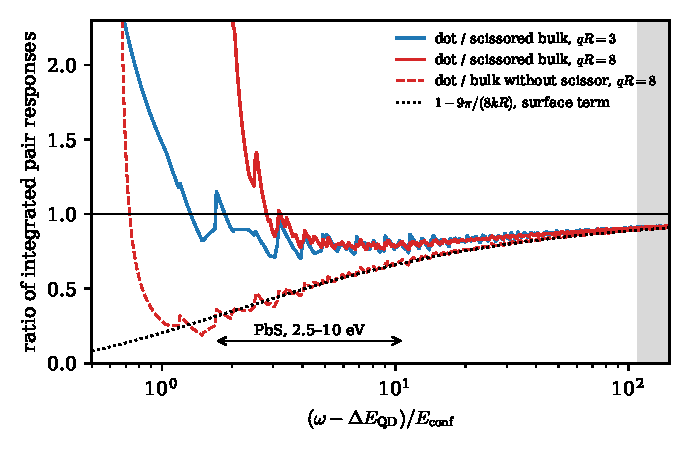
\includegraphics[width=0.85\linewidth]{figures/ch16/limit16_3b.pdf}
\captionof{figure}{Pair response of a hard-walled spherical dot, integrated from its gap up to $\omega$, divided by the same integral of the bulk response with the scissored gap, against $(\omega - \Delta E_{\mathrm{QD}})/E_{\mathrm{conf}}$, for $qR = 3$ (blue) and 8 (red). Model: envelopes of \cref{eq:16.3-gap}, equal electron and hole masses, the band-edge cell factor common to dot and bulk; the direction of $\vect{q}$ averaged. Dashed: the bulk without the scissor at $qR = 8$. Dotted: $1 - 9\pi/(8kR)$, the surface term of the level count of a sphere at $q \to 0$, with $k$ the envelope momentum. Arrow: the range of deposits of PbS dots \SI{3.3}{nm} across, 2.5 to \SI{10}{eV} with $E_{\mathrm{conf}} = \SI{0.79}{eV}$ ($qR \ge 7.5$ there). Gray: the ratios for $qR = 3$ and 8 both within \SI{10}{\percent} of one, above 109 confinement energies ($kR \ge 33$).}\label{fig:16-limit-qd}
\par}
\smallskip
Between 3 and 11 confinement energies above the gap, 3.6 to \SI{10}{eV} for these dots, the hard wall removes states near the surface and the dot carries 0.76 to 1.03 of the scissored bulk response at $qR = 8$ (0.70 to 0.97 at $qR = 3$). The deficit relative to the scissored bulk is set by $kR$ and not by $qR$. Nearer the gap the discrete levels dominate the cumulative ratio, which reaches 2.4 to 66 at $qR = 8$.
\end{limitbox}

The deficit comes from the surface. A wavefunction that must vanish at the surface is depleted within about a wavelength of it, and the number of levels of a sphere below momentum $k$ is $Vk^3/6\pi^2 - Sk^2/16\pi$, with $V$ and $S$ its volume and surface. The second term removes the fraction $9\pi/8kR$ of the bulk count, and the scissor, which shifts the bulk by a fixed energy, corrects only at order $1/(kR)^2$. Between 3 and 11 confinement energies above the gap the model lies 15 to \SI{30}{\percent} below the scissored bulk over most of the range. A real dot has surface atoms and ligands with states of their own, and its wall is not infinitely high. For a real dot the hard wall therefore overstates the depletion, and the measured bulk-like optical response above \SI{2.5}{eV} points to a smaller depletion.

\paragraph{Absorption and the depolarization factor.} A dark photon of mass $m_\phi$ near the dot gap has a reduced wavelength $1/m_\phi v$ of about \SI{0.2}{mm} at \SI{1}{eV}. Over a dot the dark-photon field is uniform, and a dot in a host is a dielectric sphere in a uniform field. Inside, the potential is $-E_{\mathrm{in}}r\cos\theta$; outside it is $-E_0r\cos\theta$ plus a dipole term $\propto\cos\theta/r^2$. Continuity of the potential and of $\varepsilon\,\partial_r\phi$ at $r = R$ gives $E_{\mathrm{in}} = 3\varepsilon_{\mathrm{out}}E_0/(\varepsilon_{\mathrm{in}} + 2\varepsilon_{\mathrm{out}})$, with $\varepsilon_{\mathrm{in}}$ and $\varepsilon_{\mathrm{out}}$ the dielectric functions of the dot and of the host at $\omega = m_\phi$. The polarization of a dilute set of these dielectric spheres gives the Maxwell Garnett dielectric function $\varepsilon_{\mathrm{eff}} = \varepsilon_{\mathrm{out}}[1 + 3\varphi_{\mathrm{QD}}b/(1 - \varphi_{\mathrm{QD}}b)]$, $b = (\varepsilon_{\mathrm{in}} - \varepsilon_{\mathrm{out}})/(\varepsilon_{\mathrm{in}} + 2\varepsilon_{\mathrm{out}})$. To first order in $\varphi_{\mathrm{QD}}$ and for a real $\varepsilon_{\mathrm{out}}$, $\Imag(-1/\varepsilon_{\mathrm{eff}}) = (3\varphi_{\mathrm{QD}}/\varepsilon_{\mathrm{out}})\Imag b = 9\varphi_{\mathrm{QD}}\Imag\varepsilon_{\mathrm{in}}/|\varepsilon_{\mathrm{in}} + 2\varepsilon_{\mathrm{out}}|^2$, the loss function that enters \cref{eq:10.7-dp}. Per unit mass of dot material this loss function replaces the bulk loss function $\Imag\varepsilon_{\mathrm{in}}/|\varepsilon_{\mathrm{in}}|^2$ that a rescaling of the measured photon cross-section with the dot's own $\varepsilon$ uses~\cite[Eq.~(16)]{blanco2023dark}. The two loss functions differ by the depolarization factor
\begin{equation}
  \frac{9\,|\varepsilon_{\mathrm{in}}|^2}{|\varepsilon_{\mathrm{in}} + 2\varepsilon_{\mathrm{out}}|^2} > 1 \iff |\varepsilon_{\mathrm{in}}|^2 > \frac{\varepsilon_{\mathrm{out}}}{2}\,\bigl(\Real\varepsilon_{\mathrm{in}} + \varepsilon_{\mathrm{out}}\bigr) .
  \label{eq:16.3-depol}
\end{equation}
The criterion follows from expanding $|\varepsilon_{\mathrm{in}} + 2\varepsilon_{\mathrm{out}}|^2 = |\varepsilon_{\mathrm{in}}|^2 + 4\varepsilon_{\mathrm{out}}\Real\varepsilon_{\mathrm{in}} + 4\varepsilon_{\mathrm{out}}^2$. The factor tends to 9 when $|\varepsilon_{\mathrm{in}}| \gg \varepsilon_{\mathrm{out}}$, equals one when dot and host are the same medium, and falls below one when $|\varepsilon_{\mathrm{in}}|$ is of order one; for a real $\varepsilon_{\mathrm{in}}$ it exceeds one exactly when $\varepsilon_{\mathrm{in}} > \varepsilon_{\mathrm{out}}$.

\begin{workedexample}{The depolarization factor of a PbS dot in a glass}\label{we:16-depol}
Take a PbS dot in fused silica. Below the bulk gap, at \SI{3.5}{\micro m} (\SI{0.354}{eV}), the dispersion formula of Zemel et al.~\cite{zemel1965electrical} gives $\varepsilon_{\mathrm{in}} = 17.63$, real, and Malitson's fit for silica~\cite{malitson1965interspecimen} gives $\varepsilon_{\mathrm{out}} = 1.977$, both as tabulated in Ref.~\cite{polyanskiy2024refractiveindex}. The field inside the dot is $3\varepsilon_{\mathrm{out}}/(\varepsilon_{\mathrm{in}} + 2\varepsilon_{\mathrm{out}}) = 0.275$ of the field in the glass, against $1/\varepsilon_{\mathrm{in}} = 0.0567$ in bulk PbS, and the depolarization factor is
\begin{equation*}
  \frac{9 \times 17.63^2}{(17.63 + 2\times1.977)^2} = 6.00 .
\end{equation*}
The factor depends little on the exact value of $\varepsilon_{\mathrm{in}}$: $\Real\varepsilon_{\mathrm{in}} = 10$ gives 4.62 and 25 gives 6.71. Wherever $|\varepsilon_{\mathrm{in}}|$ is large, as near the absorption edge of a dot, the bulk formula therefore underestimates the absorption rate by a factor of 4.6 to 6.7. At \SI{5}{eV} silica has $\varepsilon_{\mathrm{out}} = 2.276$. If $\varepsilon_{\mathrm{in}}$ there were $1 + \ii$, an illustrative value near one, the factor would be 0.566, and the bulk formula would overestimate the rate; for $\varepsilon_{\mathrm{in}} = 3 + 3\ii$ it would be 2.45.
\end{workedexample}

Over 2.5 to \SI{10}{eV}, the range of Blanco et al., it is not known whether the depolarization factor is above or below one. The size and even the sign of the depolarization correction need the dielectric function $\varepsilon_{\mathrm{in}}(\omega)$ of real dots of the size used, measured or computed. With it, \cref{eq:16.3-depol} is a one-line evaluation.
